\section{Grundlagen der Steuerungstechnik}
\subsection{Sensoren}
Sensoren erfassen Messgrößen der Umwelt und wandeln diese in elektrische, hydraulische oder pneumatische Ausgangsgrößen um. Hierzu werden physikalische, chemische oder biologische Effekte genutzt. Das Ausgangssignal kann analog (z.B. PTC-Temperatursensor) oder digital (z.B. Hallsensor) ausgegeben werden. Moderne Sensoren besitzen meistens zusätzlich Wandler, Verstärker und Signalvorverarbeitungselemente. Sie werden auch als integrierte Sensoren bezeichnet. \autocite[vgl.][389 \psqq]{Hering2021} \\
Es gibt eine Vielzahl verschiedener Sensoren. In diesem Assign\-ment wird nur auf die für die Bohrvorrichtung benötigten Sensoren eingegangen. Hierbei müssen die Anfangs- und Endpositionen der Zylinder erfasst werden. Das kann mechanisch, kapazitiv, induktiv, über Widerstandsänderungen, mithilfe des Hall-Effekts, akustisch, optisch oder magnetisch erfolgen. \autocite[vgl.][394\psqq]{Hering2021} \\
Magnetische Zylindersensoren stellen die einfachste und effektivste Variante dar, um die Endanschläge des Zylinders zu erfassen.
\begin{figure}[H]
   \centering
    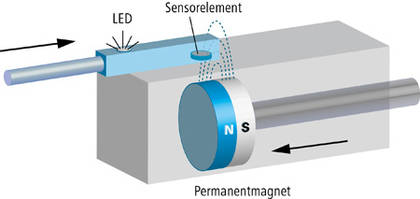
\includegraphics[scale=0.7]{Bilder/magnetischer_Zylinderschalter.jpg}
    \caption[magnetischer Sensor]{magnetischer Sensor
    \footnotemark}
    \label{fig:magSensor}
\end{figure}
\footnotetext{\cite{Magnetsensor}}
In Abbildung \ref{fig:magSensor} ist die Funktionsweise eines solchen Sensors dargestellt. Beim Erreichen der jeweiligen Position erfolgt durch den magnetischen Kolben eine Magnetfeldänderung. Diese wird vom Sensorelement registriert. Je nach Schaltlogik gibt der integrierte Sensor ein High oder Low als Ausgangsgröße aus, welches von einer Steuerungsanlage verarbeitet werden kann. \autocite[vgl.][]{Magnetsensor}
%-----------------------------------------------------------------------------------------------
%-----------------------------------------------------------------------------------------------
\subsection{Aktuatoren}
Aktuatoren (mittellateinisch actuare = sich betätigen, auch Aktor genannt \autocite{Aktuator}) bestehen im Allgemeinen aus einem Energiesteller, der aus der Stellgröße zusammen mit einer Hilfsenergie einen Energiefluss erzeugt. Dieser wird durch einen Energiewandler in eine andere physikalische Größe, meist eine mechanische Bewegung, überführt.\autocite[vgl.][30\psqq]{Heimann2016}\\
Wie bei den Sensoren gibt es auch bei den Aktuatoren die unterschiedlichsten Arten, welche auf verschiedenen Wirkprinzipien beruhen. Hierauf kann im Rahmen des Assign\-ments nicht näher eingegangen werden.\\
Für die Bohreinrichtung wird zum einen ein Elektromotor benötigt. Dieser wandelt einen elektrischen Strom in eine rotatorische Bewegung um. Zum anderen werden zwei fluidische Aktoren benötigt, die die Bewegung einer Flüssigkeit oder eines Gases in eine mechanisch translatorische Bewegung umwandeln. Zum Einsatz kommen laut Aufgabenstellung zwei doppelt wirkende Pneumatikzylinder mit einseitiger Kolbenstange und elektromagnetischer Betätigung.
\begin{figure}[H]
   \centering
    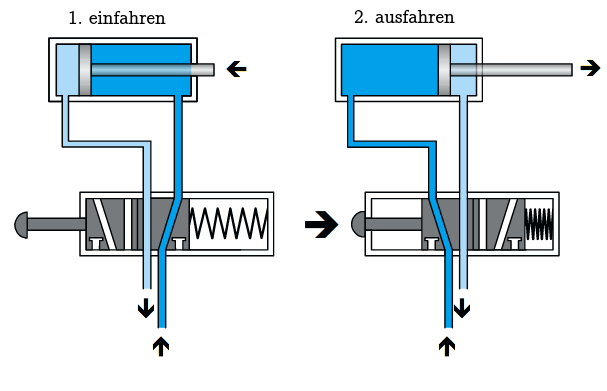
\includegraphics[scale=0.5]{Bilder/Zylinder.png}
    \caption[doppeltwirkender Pneumatikzylinder]{Funktionsweise eines doppeltwirkenden Pneumatikzylinders
    \footnotemark}
    \label{fig:Zylinder}
\end{figure}
\footnotetext{\cite[in Anlehnung an:][]{Festo2000}}
In Abbildung \ref{fig:Zylinder} wird die Ansteuerung der Zylinder mit einem mechanisch betätigtem 5/2-Wegeventil dargestellt. Links wird der Einfahrprozess ersichtlich, die rechte Darstellung zeigt den Ausfahrvorgang. Die dunkelblau eingefärbten Leitungen sind jeweils mit Druck beaufschlagt, das bewirkt eine Bewegung des Kolbens aufgrund eines Differenzdruckes. Eine messtechnische Erfassung des Druckes ist ebenso möglich. Pneumatisch gesteuerte Aktuatoren weisen eine schlechte Regelbarkeit der \mbox{(Ausfahr-)Geschwindigkeit} auf. Deshalb sind die Zylinder in der Aufgabenstellung zusätzlich mit einer Ölbremseinheit ausgestattet. \autocite[vgl.][54\psq]{Heimann2016}
%-----------------------------------------------------------------------------------------------
%-----------------------------------------------------------------------------------------------
\subsection{Speicherprogrammierbare Steuerung}
Eine \ac{sps} ist eine programmierbare elektronische Einheit, welche Maschinen und Anlagen steuern und regeln kann. Ihr Vorgänger ist die \ac{vps}. Im Unterschied zur \ac{sps} wurde der Programmablauf durch eine feste Verdrahtung der Logikbausteine realisiert. Dadurch ist die \ac{vps} bei komplexen Systemen sehr aufwändig zu realisieren. Zusätzlich ist die Anpassung an veränderte Bedingungen der Steuerung nicht oder nur schwer möglich.\autocite[vgl.][755]{Hering2021}
\begin{figure}[H]
   \centering
    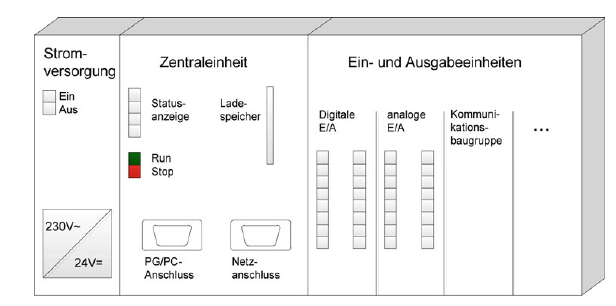
\includegraphics[scale=0.75]{Bilder/SPS-Aufbau.png}
    \caption[Aufbau einer SPS]{Aufbau einer SPS
    \footnotemark}
    \label{fig:SPS_Aufbau}
\end{figure}
\footnotetext{\cite{Boege2021}}
Der grundlegende Aufbau einer \ac{sps} besteht in der Minimalausführung aus einer Stromversorgung, einer Zentraleinheit und einer Ein- und Ausgabeeinheit (siehe Abbildung \ref{fig:SPS_Aufbau}). Die Stromversorgungseinheit wandelt die Netzspannung, meist 230 V Wechselspannung, in 24V Gleichspannung um. Die Zentraleinheit ist für die Verarbeitung und Speicherung des Ablaufprogrammes zuständig. Zusätzlich kann ein PC angeschlossen werden, um Anwenderprogramme einzulesen oder Fehler zu suchen. An der Ein- und Ausgabeeinheit werden die Sensoren und Aktuatoren angeschlossen. Zusätzlich kann die Einheit mit Kommunikationsmodulen, z.B. einem Datenbussystem oder einer WLAN-Einheit erweitert werden.\autocite[vgl.][1497\psq]{Boege2021} Die Programmbearbeitung erfolgt zyklisch. \glqq Jeder Zyklus beginnt mit dem Einlesen der aktuellen Signalzustände der Eingänge [...] und endet mit der Ausgabe der Signale an die Ausgänge [...]\grqq{}.\autocite[13]{Wellenreuther2005} Die benötigte Zeit für einen Durchlauf wird auch als Zykluszeit bezeichnet. Diese muss den Echtzeitbedingungen der \ac{sps} entsprechend ausreichend klein sein.\autocite[vgl.][13]{Wellenreuther2005}
%-----------------------------------------------------------------------------------------------
%-----------------------------------------------------------------------------------------------
\subsection{CoDeSys}
 \ac{codesys} ist eine Entwicklungsumgebung zur Programmierung und Simulation von SPS-Steuerungen.\autocite[vgl.][1]{CODESYS2004} Für das Assignment wird die Version V3.5 SP17 Patch 2, 64-bit in einer virtuellen Maschine (Host: Fedora 33, KDE Plasma, Gast: Windows 10 Pro, Version 20H2) verwendet.\\
\ac{codesys} bietet die Möglichkeit, die Programmierung in unterschiedlichen Sprachen umzusetzen. \acp{st}, \ac{as}, \ac{fup}, \ac{kop}, \ac{awl} und \ac{cfc} sind die zur Auswahl stehenden Programmiersprachen. \ac{st} ist eine textbasierte Implementierungssprache, alle anderen Sprachen verwenden einen grafischen Editor. Zusätzlich kann die Syntax und der Quellcode auf Fehler überprüft werden. \autocite[vgl.][Kapitel \glqq Programmiersprachen und ihre Editoren\grqq{} und \glqq Befehl 'Code erzeugen'\grqq{}]{manCODESYS}\\
In Abbildung \ref{fig:Oberfl_Codesys}, Seite \pageref{fig:Oberfl_Codesys} ist die Benutzeroberfläche von \ac{codesys} abgebildet. Unter (1) ist der Gerätebaum und -editor zu sehen. Die Datei \glqq PLC\_PRG (PRG)\grqq{} ist das Hauptprogramm. Bereich (2) und (3) stellen den eigentlichen Editorbereich dar. Der obere Abschnitt ist ein einfacher Texteditor (2). Hier sind unter anderem die lokalen Variablen der Funktionsbausteine sowie Ein- und Ausgänge der im unteren Bereich zu sehenden grafischen Darstellung der Schrittkette deklariert. Der grafische Editor (3) besteht aus einzelnen Netzwerken, die jeweils einen einzelnen Schritt darstellen. Im Bereich (4) können die einzelnen Operatoren und Funktionsbausteine ausgewählt werden. Bei der Erstellung einer Simulation befinden sich in diesem Bereich auch die einzelnen Steuerungselemente wie z.B. Lampen oder Schalter. \autocite[vgl.][Kapitel \glqq Ihr erstes CODESYS-Programm\grqq{} sowie \glqq Gerätebaum und Geräteeditor\grqq{}]{manCODESYS}
\begin{figure}[H]
   \centering
    \includegraphics[scale=0.53]{Bilder/Oberfläche-Codesys.png}
    \caption[Benutzeroberfläche CoDeSys]{Benutzeroberfläche CoDeSys mit geöffnetem Projekt (eigener Entwurf)}
    \label{fig:Oberfl_Codesys}
\end{figure}
%-----------------------------------------------------------------------------------------------
%-----------------------------------------------------------------------------------------------
\subsection{ISO/OSI-Referenzmodell}
Das \ac{osi}-Referenzmodell wurde von der \ac{iso} für den  einheitlichen Aufbau von Netzwerken und deren Schnittstellendefinition entworfen. Es umfasst sieben Schichten, diese sind in Abbildung \ref{fig:OSI}, Seite \pageref{fig:OSI} dargestellt.\autocite[vgl.][209]{Heimann2016} Die Daten gelangen vom Endsystem A, angefangen in Schicht sieben, schrittweise abwärts bis zur Schicht eins, wo die Daten physikalisch übertragen werden. Im Endsystem B gelangen die Daten schrittweise von Schicht eins aufwärts bis zur Anwendungsschicht.\autocite[vgl.][]{OSI}
\begin{figure}[H]
   \centering
    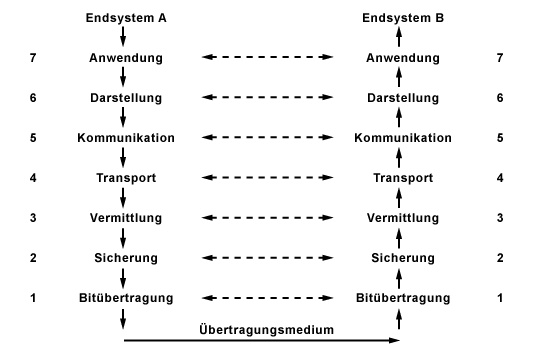
\includegraphics[scale=0.9]{Bilder/OSI-Schichtenmodell.png}
    \caption[ISO/OSI-Referenzmodell]{ISO/OSI-Referenzmodell nach ISO/IEC 7498 1:1994 \footnotemark}
    \label{fig:OSI}
\end{figure}
\footnotetext{\cite{OSI}}
Nicht alle Schichten müssen zwangsläufig verwendet werden. So sind in den Kommunikationssystemen der Automatisierung meistens nur die Schichten eins, zwei und sieben vorhanden. In der Bitübertragungsschicht werden die elektrischen, mechanischen und funktionalen Anforderungen festgelegt. So werden z.B. die Taktrate, Leitungscodierungen oder Steckerform festgelegt. In der Sicherungsschicht werden die Adressierung, Fehlererkennungsmechanismen und Maßnahmen zur sicheren Übertragung von Datenpaketen festgelegt. Die siebte Schicht stellt das Mensch-Maschine-Interface dar. Hier wird dem Anwender erst ermöglicht, die Maschine oder Anlage zu bedienen. Eine Dateneingabe und -ausgabe kann ebenso erfolgen. \autocites[vgl.][209]{Heimann2016}[vgl.][]{OSI}
